\documentclass[12pt]{article}
\usepackage{graphicx} % Required for inserting images
\usepackage[a4paper, total={6in, 8.5in}]{geometry}
\usepackage{amsmath}
\usepackage{amssymb}
\usepackage{graphicx}
\usepackage{comment}
\usepackage{framed}
\usepackage{hyperref}
\usepackage{float}
\usepackage{subcaption}
\usepackage{varioref}
\usepackage{tikz}
\usepackage[shortlabels]{enumitem}
\usepackage{xcolor}
\usepackage{mathrsfs}
\usepackage{amsthm}
\usepackage{graphics}
\usepackage[most]{tcolorbox}
\usepackage{xcolor}
\usepackage{mathtools}
\usepackage{cancel}
\usepackage{mathdots}
\usepackage{dsfont}
\usepackage{cancel}
\usepackage{minted}
\setminted{fontsize=\footnotesize}
\usepackage{bbm}
\usepackage{setspace}

\newcommand\ItemImage[2][]{%
    \hfill\raisebox{\dimexpr-\height+\baselineskip}{\includegraphics[#1]{#2}}\hfill~}
\title{Working Draft: Optimal Test Design}
\author{ECON 29800 Thesis}
\date{October 2026}

\newcommand{\x}{x^*}
\newcommand{\y}{y^*}
\newcommand{\W}{W^*}
\newcommand{\M}{M^*}
\renewcommand{\a}{\alpha}
\renewcommand{\b}{\beta}
\newcommand{\bgt}{p_xx+p_yy=m}
\newcommand{\bg}{p_xx+p_yy}
\newcommand{\mbg}{m-p_xx-p_yy}
\newcommand{\xom}{x^M_1}
\newcommand{\xtm}{x^M_2}
\newcommand{\xrm}{x^M_3}
\newcommand{\xoh}{x^H_1}
\newcommand{\xth}{x^H_2}
\newcommand{\p}{\rho}
\newcommand{\U}{\overline{U}}
\newcommand{\ds}{\displaystyle}
\newcommand{\e}{\varepsilon}
\renewcommand{\l}{\lambda}
\newcommand{\bm}{b_M}
\newcommand{\cm}{c_M}
\newcommand{\mx}{\text{max}_{x,y}}
\newcommand{\mn}{\text{min}_{x,y}}
\newcommand{\del}{\partial}
\newcommand{\pv}{\mathbf{p}}
\newcommand{\xv}{\mathbf{x}}
\newcommand{\lag}{\mathcal{L}}
\newcommand{\s}{\sigma}
\newcommand{\wv}{\boldsymbol{\omega}}
\newcommand{\w}{\omega}
\newcommand{\bbR}{\mathbb{R}}
\newcommand{\xo}{x_1^*}
\newcommand{\xt}{x_2^*}
\newcommand{\dotp}{\boldsymbol{\cdot}}
\newcommand{\ev}{\mathbf{e}}
\newcommand{\zv}{\mathbf{z}}
\newcommand{\dv}{\mathbf{d}}
\newcommand{\yv}{\mathbf{y}}
\newcommand{\bbN}{\mathbb{N}}
\newcommand{\bbQ}{\mathbb{Q}}
\newcommand{\bbZ}{\mathbb{Z}}
\newcommand{\bbP}{\mathbb{P}}
\newcommand{\bbE}{\mathbb{E}}
\newcommand{\bbV}{\mathbb{V}}
\renewcommand{\mod}{\text{mod }}
\newcommand{\<}{\langle}
\renewcommand{\>}{\rangle}

\definecolor{g}{RGB}{30, 100, 200}
\definecolor{f}{RGB}{200, 30, 100}
\definecolor{t}{RGB}{50, 150, 0}


\newtheorem{theorem}{Theorem}
\newtheorem*{theorem1*}{Theorem 1}
\newtheorem*{theorem2*}{Theorem 2}
\newtheorem*{theorem3*}{Theorem 3}
\newtheorem*{theorem5*}{Theorem 5}
\newtheorem*{theorem*}{Theorem}
\newtheorem{lemma}[theorem]{Lemma}
\newtheorem{remark}[theorem]{Remark}
\newtheorem{proposition}[theorem]{Proposition}

\onehalfspacing

\newtcolorbox{qbox}{
    colback=gray!10, % Sets the background color to a light gray
    colframe=gray!80, % Sets the frame/border color to a darker gray
    boxrule=0.7pt, % Sets the thickness of the box border
    arc=0mm, % Rounds the corners of the box
    boxsep=2pt, % Sets the distance between the border and the inner content
    left=5mm, % Adds extra space to the left side
    right=5mm, % Adds extra space to the right side
}

\newtcolorbox{abox}{
    colback=gray!0, % Sets the background color to a light gray
    colframe=gray!80, % Sets the frame/border color to a darker gray
    boxrule=0.7pt, % Sets the thickness of the box border
    arc=0mm, % Rounds the corners of the box
    boxsep=2pt, % Sets the distance between the border and the inner content
    left=5mm, % Adds extra space to the left side
    right=5mm, % Adds extra space to the right side
    breakable=true,
}


\begin{document}

\maketitle

% \begin{abstract}
%     I study the question of optimal design of a test/performance measure when candidates have adverse incentives and access to technology that allows them to `game the test' in an unobserved fashion. I show that in general, in the presence of gaming, firms may benefit from strategically misaligning tests/performance measures from their true payoffs.
% \end{abstract}

% \section{Introduction}



% \section{Prior Literature}

\section{Preliminary Model}

In this section, I introduce the economic model that formalizes the notion of testing under adverse incentives.

For now, suppose there is a Sender (he) and a Receiver (she). Broadly speaking, the Sender is the agent being evaluated who has the ability to game; the Receiver is the agent who wishes to evaluate and reward Sender's skill.


There are $D \geq 2$ axes representing independent dimensions of ability. A (composite) `skill' is a vector $a \in \bbR ^D_+$.\\

\noindent From a skill $a$, Receiver obtains payoff $\pi_R \equiv \pi_0+\<r,a\>$, where $\<\cdot, \cdot\>$ is the standard Euclidean inner product and $r \in \bbR^D_+$.

Receiver chooses a `test' $g \in S^{D-1}_+$, with a resultant test score of is $\<g,a\>$. Receiver then observes a random binary score $H \sim \text{Bernoulli}(\<g,a\>)$. She \textbf{only observes $H$}, not $a$. If $H = 1$, she compensates Sender with $W$ dollars for a good performance; otherwise, she does not pay Sender. So, her optimization problem is $$\max_g \ \<r,a(g)\> - \bbE[W \cdot H(g)]$$ for a particular $a(g)$ that depends on Sender's optimization problem.\\

\noindent
Sender's goal is to exhibit high skill level $a \in \bbR^D_+$ to Receiver. He observes $g$ and $W$, and he obtains linear utility from his expected compensation $\bbE[W \cdot H]$, where $H \sim \text{Bernoulli}(\<g,a\>)$. He can exhibit this skill level in two ways:
\begin{itemize}[nosep]
    \item through \textbf{true improvements} $a_t \in \bbR ^D_+$, and
    \item through \textbf{fake manipulations} $a_f \in \bbR^D_+$ of her skill.
\end{itemize}

Then, his skill level is $a=a_t+a_f$. He faces a quadratic cost $$C(a_t,a_f)=\dfrac 1 2\left(a_{t,1}^2+\dots+a_{t,D}^2+s_1a_{f,1}^2+\dots +s_Da_{f,D}^2\right),$$ where $s_1,s_2,\dots,s_D$ represent the relative cheapness of faking. We will often assume $s_k \leq 1$ for all $k$, which would make gaming cheaper on the margin. His optimization problem is $$\max_{a_t,a_f} \ \bbE[W \cdot H]-C(a_t,a_f).$$

\noindent To sum up, the chronology of the game is as follows.
Before the game starts:
\begin{itemize}[nosep]
    \item Receiver has a payoff $\pi_R(\cdot)=\pi_0+\<r,\cdot\>$, which is parameterized by her `preferred direction' $r$.
    \item Sender has a cost function $C(\cdot,\cdot)$, which is parameterized by $s_1,s_2,\dots,s_D$. 
\end{itemize}

\noindent The game progresses as follows: 
\begin{itemize}[nosep]
    \item Receiver announces the test $g$ and she \textit{must} commit to it. 
    \item Sender observes $g$ and plays his optimal $(a_t^*,a_f^*)$. 
    \item Receiver observes the realized value of $H \sim \text{Bernoulli}(\<g,a^*_t+a_f^*\>)$. 
    \begin{itemize}[nosep]
        \item Receiver only cares about Sender's true skill, so her payoff is actually $\pi_R(a_t^*)=\pi_0+\<r,a_t^*\>$. 
    \end{itemize}
    \item Sender obtains his compensation from Receiver if $H=1$, and nothing if $H=0$.
\end{itemize}

\section{Solving the Model}

We begin by backward induction and solve Sender's problem for a given choice of $g$: $$\max_{a_t,a_f} \ \bbE[W \cdot H]-C(a_t,a_f),$$ with FOCs for skills $k=1,2,\dots,D$: $$[a_{f,k}]:a_{f,k}^*=\dfrac{Wg_k}{s_k}, \quad [a_{t,k}]:a_{t,k}^*=Wg_k.$$ Three facts follow immediately from this result:
\begin{itemize}[nosep]
    \item $a_{t,k}^* =s_k \cdot a_{f,k}^* \leq a_{f,k}^*$.
    \item $a_t^* \parallel g$.
    \item $a_t^*$ and $a_f^*$ will \textit{not} be parallel unless all skills are equally expensive to game. $a_f^*$ will tend to point towards cheaper skills (i.e. it will be inflated relative to $a_t^*$ in the directions where $s_k$ is lower).\\
\end{itemize}

\noindent Geometrically, if $g=(\tfrac{\sqrt 2}2,\tfrac{\sqrt 2}2)$, $s=(1, \tfrac 1 2)$, and $W=2$, Sender's optimal responses look like this:

\begin{center}
\begin{tikzpicture}[scale=2.5, >=stealth]
% g = (cos 45, sin 45), s = (1, 0.5), W = 2
    \pgfmathsetmacro{\gone}{cos(45)}
    \pgfmathsetmacro{\gtwo}{sin(45)}
    \pgfmathsetmacro{\sone}{1}
    \pgfmathsetmacro{\stwo}{0.5}
    \pgfmathsetmacro{\W}{2}

    % a_t^* = W g        (parallel to g)
    \pgfmathsetmacro{\atone}{\W*\gone}
    \pgfmathsetmacro{\attwo}{\W*\gtwo}
    % a_f^* = W S^{-1} g  (tilts toward cheap-to-game axis)
    \pgfmathsetmacro{\afone}{\W*\gone/\sone}
    \pgfmathsetmacro{\aftwo}{\W*\gtwo/\stwo}

    % axes (positive quadrant only)
    \draw[->] (0,0) -- (3.2,0) node[right] {$x$};
    \draw[->] (0,0) -- (0,3.2) node[above] {$y$};

    % g: unit vector at 45 degrees
    \draw[dotted, very thick, g] (0,0) -- (45:4) node[below right] {$\parallel g$};

    % a_f^*: tilts toward the cheaper-to-game axis (y)
    \draw[->, very thick, f] (0,0) -- (\afone,\aftwo)
      node[above right] {$a_f^*$};

    % a_t^* = W g : lies on the test line
    \draw[->, very thick, t] (0,0) -- (\atone,\attwo)
      node[below right] {$a_t^*$};

\end{tikzpicture}
\end{center}

\noindent
Substituting Sender's optimum into Receiver's problem gives $$\max_{g} \ \pi_0+W\sum_k r_kg_k-W^2\sum_k\dfrac{s_k+1}{s_k}g_k^2,$$ with FOCs for $k=1,2,\dots,D$:
$$[g_k]:Wr_k=2W^2\dfrac{s_k+1}{s_k}g_k,$$ which gives $$g_k^*=\dfrac{s_k}{2(s_k+1)W}\cdot r_k.$$ Again, unless all skills are equally expensive to game, $g^*$ is \textit{not} parallel to $r$.\\

Dividing $g_k^*$ by $g_j^*$ gives $$\underbrace{\dfrac{g_k^*}{g_j^*}}_{\text{Sender's } MRS_{k,j}}=\underbrace{\dfrac{s_k/(s_k+1)}{s_j/(s_j+1)}}_{\text{share of true improvement along axis } k \text{ vs } j} \times\underbrace{\dfrac{r_k}{r_j}}_{\text{Receiver's } MRS_{k,j}}$$ There are two interpretations of this formula:
\begin{itemize}[nosep]
    \item Receiver should equate Sender's MRS to her MRS, scaled by the share of true improvement along each axis.
    \item Receiver should choose the test that equates Sender's MRS to true relative cost of true improvement, scaled by the weights she places on those axes (this is like an MRS = Price condition).\\
\end{itemize}

\noindent Geometrically, when $a_t^*=Wg$, setting $g\parallel r$ perfectly aligns true skill with $r$. But fake manipulation points towards the more gameable axis so the compensation for fake skill rises:

\begin{figure}[htbp]
  \centering
  \begin{minipage}{0.45\textwidth}
    \centering
    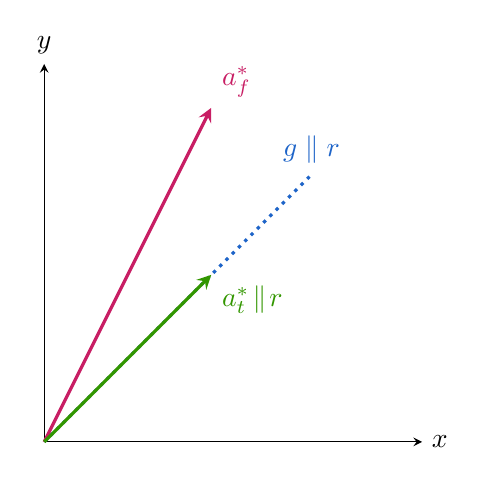
\begin{tikzpicture}[scale=1.5, >=stealth]
      \pgfmathsetmacro{\rone}{cos(45)} \pgfmathsetmacro{\rtwo}{sin(45)}
      \pgfmathsetmacro{\gone}{cos(45)} \pgfmathsetmacro{\gtwo}{sin(45)}
      \pgfmathsetmacro{\sone}{1} \pgfmathsetmacro{\stwo}{0.5}
      \pgfmathsetmacro{\W}{2}
      % a_t = W g  (parallel to g = r)
      \pgfmathsetmacro{\atone}{\W*\gone} \pgfmathsetmacro{\attwo}{\W*\gtwo}
      % a_f = W S^{-1} g  (tilts toward cheap-to-game axis)
      \pgfmathsetmacro{\afone}{\W*\gone/\sone} \pgfmathsetmacro{\aftwo}{\W*\gtwo/\stwo}

      \draw[->] (0,0) -- (3.2,0) node[right] {$x$};
      \draw[->] (0,0) -- (0,3.2) node[above] {$y$};
      \draw[dotted, very thick, g] (0,0) -- (3.2*\gone,3.2*\gtwo) node[above] {$g\parallel r$};
      \draw[->, very thick, f] (0,0) -- (\afone,\aftwo) node[above right] {$a_f^*$};
      \draw[->, very thick, t] (0,0) -- (\atone,\attwo) node[below right] {$a_t^*\!\parallel\! r$};
    \end{tikzpicture}
  \end{minipage}
  \hfill
  \begin{minipage}{0.45\textwidth}
    \centering
    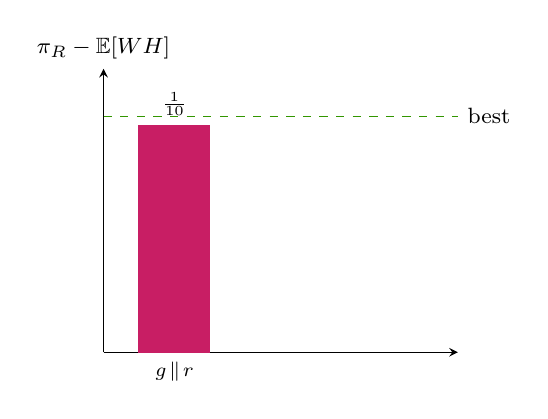
\begin{tikzpicture}[scale=1.5, >=stealth]
      \pgfmathsetmacro{\hA}{1/10*19.2}    % 1.92
      \pgfmathsetmacro{\hopt}{5/48*19.2}  % 2.00
      \draw[->] (0,0) -- (0,2.4) node[above] {\footnotesize $\pi_R-\mathbb{E}[WH]$};
      \draw[->] (0,0) -- (3,0);
      \draw[dashed, t] (0,\hopt) -- (3,\hopt) node[right, black] {\footnotesize best};
      \filldraw[f] (0.3,0) rectangle (0.9,\hA);
      \node[below] at (0.6,0) {\scriptsize $g\!\parallel\!r$};
      \node[above] at (0.6,\hA) {\scriptsize $\tfrac{1}{10}$};
    \end{tikzpicture}
  \end{minipage}

  \caption{The true skill is aligned, but Receiver pays Sender much more for fake skill.}
  \label{fig:gparallelr}
\end{figure}

Receiver's optimal test is what might be called `strategic misalignment': she should tilt the test towards the harder-to-game axis. While this tilts $a_t^*$ away from $r$, it reduces the cost she wastes on gamed skill $a_f^*$: \newpage

\begin{figure}[htbp]
  \centering
  \begin{minipage}{0.46\textwidth}
    \centering
    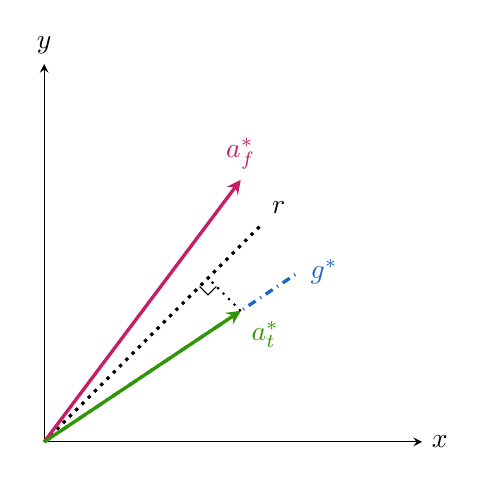
\begin{tikzpicture}[scale=1.5, >=stealth]
      \pgfmathsetmacro{\rone}{cos(45)} \pgfmathsetmacro{\rtwo}{sin(45)}
      \pgfmathsetmacro{\gone}{3/sqrt(13)} \pgfmathsetmacro{\gtwo}{2/sqrt(13)}
      \pgfmathsetmacro{\sone}{1} \pgfmathsetmacro{\stwo}{0.5}
      \pgfmathsetmacro{\W}{2}
      \pgfmathsetmacro{\atone}{\W*\gone} \pgfmathsetmacro{\attwo}{\W*\gtwo}
      \pgfmathsetmacro{\afone}{\W*\gone/\sone} \pgfmathsetmacro{\aftwo}{\W*\gtwo/\stwo}
      \pgfmathsetmacro{\projt}{\atone*\rone + \attwo*\rtwo}
      \pgfmathsetmacro{\footone}{\projt*\rone} \pgfmathsetmacro{\foottwo}{\projt*\rtwo}
      \pgfmathsetmacro{\m}{0.1}

      \draw[->] (0,0) -- (3.2,0) node[right] {$x$};
      \draw[->] (0,0) -- (0,3.2) node[above] {$y$};
      \draw[dotted, very thick] (0,0) -- (2.6*\rone,2.6*\rtwo) node[above right] {$r$};
      \draw[dash dot, very thick, g] (0,0) -- (2.6*\gone,2.6*\gtwo) node[right] {$g^*$};
      \draw[->, very thick, f] (0,0) -- (\afone,\aftwo) node[above] {$a_f^*$};
      \draw[->, very thick, t] (0,0) -- (\atone,\attwo) node[below right] {$a_t^*$};
      \draw[dotted, thick] (\atone,\attwo) -- (\footone,\foottwo);
      \draw[thin]
        (\footone-\m*\rone, \foottwo-\m*\rtwo) --
        (\footone-\m*\rone+\m*\rtwo, \foottwo-\m*\rtwo-\m*\rone) --
        (\footone+\m*\rtwo, \foottwo-\m*\rone);
    \end{tikzpicture}
  \end{minipage}
  \hfill
  \begin{minipage}{0.46\textwidth}
    \centering
    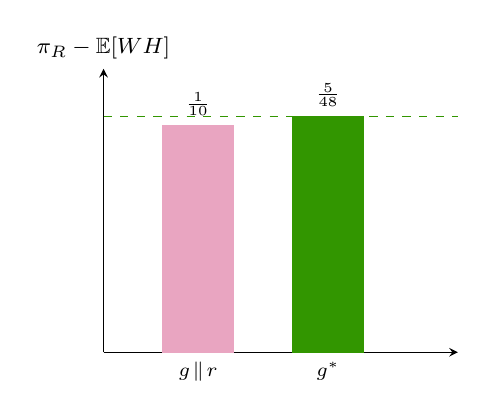
\begin{tikzpicture}[scale=1.5, >=stealth]
      \pgfmathsetmacro{\hA}{1/10*19.2}    % 1.92  (g || r)
      \pgfmathsetmacro{\hC}{5/48*19.2}    % 2.00  (g*)
      \pgfmathsetmacro{\hopt}{5/48*19.2}
      \draw[->] (0,0) -- (0,2.4) node[above] {\footnotesize $\pi_R-\mathbb{E}[WH]$};
      \draw[->] (0,0) -- (3,0);
      \draw[dashed, t] (0,\hopt) -- (3,\hopt);
      \filldraw[f!40] (0.5,0) rectangle (1.1,\hA);
      \filldraw[t] (1.6,0) rectangle (2.2,\hC);
      \node[below] at (0.8,0) {\scriptsize $g\!\parallel\!r$};
      \node[below] at (1.9,0) {\scriptsize $g^*$};
      \node[above] at (0.8,\hA) {\scriptsize $\tfrac{1}{10}$};
      \node[above] at (1.9,\hC) {\scriptsize $\tfrac{5}{48}$};
    \end{tikzpicture}
  \end{minipage}

  \caption{Tilting $g$ towards the harder-to-game skill reduces total gaming, offsetting the loss from misalignment.}
  \label{fig:gstar}
\end{figure}

\noindent
We summarize with two propositions, both of which are immediate consequences of the math in this section.

\begin{proposition}
    If faking is not possible (i.e., as $s_k\to \infty$ for all $k$), Receiver's optimal test is $g \parallel r$. That is, misalignment is only beneficial in the presence of faking.
\end{proposition}

\begin{proposition}
    Strategic misalignment benefits Receiver if and only if there is heterogeneity in $s_k$.
\end{proposition}

\section{Model Extensions}

\noindent We first talk about two forms of uncertainty that exist in the problem.

\subsection{Sender Uncertainty in $g$}

Suppose Receiver is allowed to announce a distribution $\nu$ over tests $g$. Then Sender does not know $g$ exactly but he knows its distribution. But note that his objective is completely linear in $g$, meaning this is equivalent to optimizing as a response to the deterministic test $\bbE_{\nu}[g]$.

Given this response, we backward induct to write the Receiver's problem as $$\max_{\nu} \ \bbE\left[\pi_0+W\sum_k r_k\bbE_\nu[g_k]-W^2\sum_k\dfrac{s_k+1}{s_k}\bbE_\nu[g_k] \cdot g_k\right].$$ This expression makes it clear that $\bbE_\nu[x_k]$ actually fixes Receiver's payoff as well, at $$\pi_0+W\sum_k r_k\bbE_\nu[g_k]-W^2\sum_k\dfrac{s_k+1}{s_k}\bbE_\nu[g_k]^2.$$ Therefore, any measure $\nu$ whose mean is the optimal $g$ is equally beneficial for Receiver.

\subsection{Receiver Uncertainty in $s$}

Suppose Receiver doesn't know $s=(s_1,\dots,s_D)$ exactly but she believes it follows $s \sim \mu$ on $(0,1]^D$. Rewriting Receiver's payoff as dependent on $g$ and $s$, we note that $\pi_R(g;s)$ is concave in $s$. Consequently, by Jensen's inequality, \begin{align*}\max_g \ \bbE_\mu[\pi_R(g;s)]&= \bbE_\mu[\pi_R(g^*,s)] \\ &\leq \pi_R(g^*,\bbE_\mu[s])\leq \max_g \ \pi_R(g,\bbE_\mu[s]).\end{align*} We generalize this finding to broader notions of informativeness that Receiver has about Sender's gaming technology: 

\begin{proposition}
    Let $V_R(\mu) \equiv \max_g \bbE_{\mu}[\pi_R(g;s)]$. If $\mu_1$ second order stochastically dominates $\mu_2$, $V_R(\mu_1) \geq V_R(\mu_2)$.
\end{proposition}

\subsection{Two Senders}

Now suppose there are two Senders $i=1,2$, and Receiver will compensate at most Sender. She will administer test $g$, and observe independent binary signals $H_i \sim \text{Bernoulli}(\<g,a^i\>)$. If $H_1>H_2$, she will compensate Sender $1$ and vice versa; if $H_1=H_2=1$, she will compensate each Sender with equal probability; if $H_1=H_2=0$, she will compensate neither Sender.

Given $g$ and $W$, Senders' optimal skill exhibition is now a strategic game, with Sender $i$'s payoff given by $$u_i(a_t^i,a_f^i; a_t^{-i}, a_f^{-i})=W \cdot \left[\bbP(H_i>H_{-i})+\tfrac 1 2\bbP(H_i=H_{-i}=1)\right]-C(a_t^i,a_f^i).$$ Beacuse Senders' signals are independent, \begin{align*}u_i&=W \cdot [\bbP(H_i=1)\bbP(H_{-i}=0)+\tfrac 1 2 \bbP(H_i=1)\bbP(H_{-i}=1)] - C(a_t^i,a_f^i)\\
&=W \cdot \<g,a_t^i+a_f^i\>(1-\<g,a_t^{-i}+a_f^{-i}\>+\tfrac 1 2\<g,a_t^{-i}+a_f^{-i}\>)-C(a_t^i,a_f^i)\\
&=W \cdot \<g,a_{t}^i+a_f^i\>(1-\tfrac 1 2\<g,a_t^{-i}+a_f^{-i}\>)-C(a_t^i,a_f^i).\end{align*}

\begin{theorem}
    Suppose $s$ is common knowledge and common to both Senders, and $$\sum_{k=1}^D Wg_k^2 \cdot \dfrac{s_k+1}{s_k}<2.$$ Then the Senders' game has a unique Nash equilibrium.
\end{theorem} 
\begin{proof}
    In any Nash equilibrium both Senders must be best responding. For Sender 1, for example, given Sender 2's exhibited skills, $$\nabla u_1(a_t^1,a_f^1; a_t^2,a_f^2)=0.$$ In particular, for each skill $k$, $$W(1-\tfrac 1 2\<g,a_t^2+a_f^2\>)g_k=a_{t,k}^1, \quad \dfrac W{s_k}(1-\tfrac 1 2\<g,a_t^2+a_f^2\>)g_k=a_{f,k}^1.$$ This shows that the best response functions are continuous, singleton-valued, and symmetric; write $B(\cdot,\cdot)$ as the best-response function.

    The functional form of the BRFs shows that they are linear in the inputs; so $B(\cdot,\cdot)$ can just be represented by an affine transformation. More precisely, writing $A^i=(a_t^i,a_f^i) \in \bbR^{2D}_+$, $$B(A^i)=b+B_LA^i$$ for a matrix $B_L$.

    Letting $m=(Wg_1, Wg_2,\dots,Wg_D,\tfrac W{s_1}g_1,\dots,\tfrac W{s_D}g_D)'$ and $\ell=(g_1,\dots,g_D,g_1,\dots,g_D)'$, we notice that $$b=m, \quad B_L= -\dfrac 1 2 m\ell^T.$$ Because $B_L$ is an outer product, its column space is spanned by $m$ so it has rank one, and in particular at most one non-zero eigenvalue corresponding to $m$: $$B_Lm=-\dfrac 1 2 m\ell^Tm=-\dfrac{1}2\ell^Tm \cdot m,$$ so the eigenvalue is $-\tfrac 1 2 \ell^Tm$. Expanding out gives $$-\dfrac 1 2 \ell^Tm=-\dfrac 1 2 \sum_{k=1}^D W g_k^2 \cdot \dfrac{s_k+1}{s_k}.$$ Whenever the sum is less than $2$, the eigenvalue is in $(-1,1)$. Since it is the only non-zero eigenvalue, $B_L$ is a contraction, implying that $B$ is a contraction mapping.

    Consequently, $B$ has a unique fixed point that serves as the unique Nash equilibrium.
\end{proof}

\noindent The bound provided in the theorem statement is not arbitrary; it is equivalent to the optimal bundle resulting in a probability $\<g,a_t^i+a_f^i\> \leq 1$.

We should note firstly that this Nash equilibrium is symmetric, and can be explicitly calculated: $$B(A)=A \iff m+B_LA=A.$$ Because $B_L$ maps into the span of $m$, we must have that $A=\a m$. This implies that $$m+\a B_Lm=\a m \iff \a m=m-\dfrac 1 2 \a m\ell^Tm \implies \a = 1-\dfrac 1 2 \a\ell^Tm.$$ Isolating $\a$ gives $$\a=\dfrac 1{1+\tfrac 1 2 \ell^T m}=\dfrac{2}{2+\sum_{k=1}^D Wg_k^2 \cdot \tfrac{s_k+1}{s_k}}.$$ Therefore, the common Nash equilibrium strategy is $$(a_t^i,a_f^i)=\dfrac{2}{2+\sum_{k=1}^D Wg_k^2 \cdot \tfrac{s_k+1}{s_k}} (Wg_1,\dots,Wg_D,\tfrac W{s_1}g_1,\dots,\tfrac W{s_D}g_D).$$ There are several notable comparisons between this and the original model:
\begin{itemize}[nosep]
    \item $a_{t}^i \propto g$ and $a_{t,k}^i =s_k a^i_{f,k}\leq a_{f,k}^i$.
    \item $a_t^i$ and $a_f^i$ are parallel if and only if all skills are equally expensive to game.
    \item $(a_t^i,a_f^i)=\tfrac{2}{2+L}(a_t^*,a_f^*)\leq (a_t^*,a_f^*)$ component-wise, where $(a_t^*,a_f^*)$ is the optimal skill in the One-Sender case.
\end{itemize}

\end{document}